\begin{figure}[H]
    \centering
        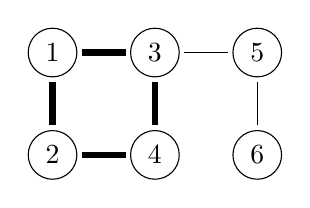
\begin{tikzpicture}[scale=1, every node/.style={circle,draw,minimum size=5mm}]
            \node (n0) at (0,1.3) {1};
            \node (n1) at (0,0) {2};
            \node (n2) at (1.3,1.3) {3};
            \node (n3) at (1.3,0) {4};
            \node (n3) at (2.6,1.3) {5};
            \node (n3) at (2.6,0) {6};
            
            \draw[line width=0.8mm, black] (0,0.375) -- (0,0.93);
            \draw[line width=0.8mm, black] (1.3,0.375) -- (1.3,0.93);
            \draw[line width=0.8mm, black] (0.375,0) -- (0.93,0);
            \draw[line width=0.8mm, black] (0.375,1.3) -- (0.93,1.3);
            \draw[very thin, black] (1.675,1.3) -- (2.23,1.3);
            \draw[very thin, black] (2.6,0.375) -- (2.6,0.93);
        \end{tikzpicture}
    \caption{Graf zawierający cykl (pogrubiona linia).}
    \label{fig:graph_cycle}
\end{figure}